%% -*- coding:utf-8 -*-



\section{Morphologie}

\author{Stefan Müller (Anke Lüdeling)}

\frame{
\frametitle{Morphologie: Material}


\citew[Kapitel~7 und 8]{Luedeling2009a}, \citew{Haspelmath2002a}




}


\frame{
\frametitle{Morphologie}


\begin{itemize}
\item Die Morphologie beschäftigt sich mit dem Aufbau komplexer Wörter.
\ea
des Brunnenkressesüppchens \citep{Luedeling2009a}
\z

Das Wort in (\mex{0}) kann man wie folgt zerteilen (((Brunnen-kresse)-süpp)-chen)-s =

Genitivform (\suffix{s}) einer kleinen (\suffix{chen}) Suppe (\emph{süpp}) mit Brunnenkresse.
\pause

\item Es gibt morphologische Bestandteile, die frei (alleine) vorkommen können (\emph{Brunnen}, \emph{Kresse},
  \emph{Suppe})
\pause
\item Es gibt morphologische Bestandteile, die nicht frei vorkommen können (\suffix{chen},
  \suffix{s}).

\pause
\item Manche Bestandteile verändern in bestimmten Umgebungen ihre Form (\emph{Suppe} vor
  \suffix{chen} $\to$ \emph{süpp}).

\pause
\item Struktur spiegelt die Bedeutung eines komplexen Ausdrucks wider.
\end{itemize}



}

\frame{
\frametitle{Wortbildung und Flexion}


Teile des Wortes machen die Bedeutung aus und könnten einen Lexikoneintrag bilden:
\emph{Brunnenkressesüppchen}.

Diese Grundform oder auch Zitierform nennt man \blaubf{Lemma}.

Die anderen Teile bestimmen die grammatischen Eigenschaften:\\
\suffix{s} = Genitiv.

Der Teil der Morphologie, der sich mit der Bildung von Lemmata beschäftigt, heißt
\blaubf{Worbildungslehre}.

Die grammatischen Formen werden in der \blaubf{Flexionsmorphologie} behandelt.


}


\subsection{Der Wortbegriff}



\frame{
\frametitle{Der Wortbegriff}

Obwohl Wörter eine zentrale Rolle in der Grammatikforschung spielen,\\
wird immer noch kontrovers diskutiert, was ein Wort ist.

Kriterien:
\begin{itemize}
\item orthographisch-graphemische
\item phonetisch-phonologische
\item morphologische
\item lexikalisch-semantische
\item syntaktische
\end{itemize}

Siehe \citew{Bussmann2002a}.

}

\subsubsection{Die orthographisch-graphemische Ebene}

\frame{
\frametitle{Die orthographisch-graphemische Ebene}

Wörter werden durch Leerzeichen voneinander getrennt.

\pause
Problem 1: Komposita im Englischen:
\eal
\ex summer school
\ex Sommerschule
\zl

\pause

Städtenamen im Deutschen:
\eal
\ex New York
\ex Berlin
\zl

}

%\begin{CJK*}{UTF8}{code2k}% Aus irgendwelchen Gründen zeigt gbsn die Punkte nicht an.


\frame{
\frametitle{Wörter sind durch Leerzeichen abgetrennt}

Problem 2: Chinesisch


%\begin{CJK*}{UTF8}{gbsn} % ist jetzt gefixt (SuSE 11.1)
近年来,``应用语言学''作为语言学的一个分支,在国内外都得到了较大的发展,但对于``什么是应用语言学'',
``应用语言学包括哪些研究领域'' 等最基本的问题,学者们却始终没有一个统一的看法。对于一门发展中的、涉及内容广泛的学科而言这是正常的,但长期下去,又会对学科的发展产生不利影响。
%\end{CJK*}

Chinesische Wörter können aus einem oder mehreren Symbolen bestehen.\\
Texte werden von oben nach unten geschrieben.\\
Auf Computern von links nach rechts.\\
Es gibt keine Leerzeichen zwischen Wörtern.

}



\frame{
\frametitle{Wörter sind durch Leerzeichen abgetrennt}

\begin{itemize}
\item Problem 3: Sprachen ohne Schriftsystem

Es gibt Sprachen, für die noch kein Schriftsystem erarbeitet wurde.

\pause

\item Problem 4: die Rechtschreibreform

Hat sich im Deutschen der Wortstatus bestimmter Buchstabenfolgen in den letzten Jahren mehrmals geändert?

\pause

Nein! Die Schriftsprache ist sekundär. 

\pause
Im besten Fall wurde das Schriftsystem von fähigen Linguisten entwickelt.
\pause

Im schlechtesten Fall spiegelt es verschiedene Stufen der historischen Entwicklung einer Sprache und diverse
Kompromisse von normierenden Institutionen wider.
\end{itemize}

}


\subsubsection{Die phonetisch-phonologische Ebene}

\frame{
\frametitle{Die phonetisch-phonologische Ebene}

Wörter sind kleinste, durch Wortakzent und Grenzsignale wie Pause, Knacklaut u.\,a.\ theoretisch
isolierbare Lautsegmente.


Das funktioniert nicht immer, da wir ohne "`Punkt und Komma"' reden.

In manchen Sprachen gibt es Phänomene wie Vokalharmonie,\\
die einen Rückschluss auf das Wortende erlauben.

}

\subsubsection{Die morphologische Ebene}

\frame{
\frametitle{Die morphologische Ebene}

Wörter sind als Grundeinheiten von grammatischen Paradigmen wie Flexion gekennzeichnet und zu
unterscheiden von den morphologisch charakterisierten Wortformen (\emph{schreiben} vs.\
\emph{schreibst}, \emph{schrieb}, \emph{geschrieben}).

\pause

Problem: Es gibt unflektierbare Wörter.


}


\subsubsection{Die lexikalisch-semantische Ebene}

\frame{
\frametitle{Die lexikalisch-semantische Ebene}

Wörter sind die kleinsten, relativ selbständigen Träger von Bedeutung,\\
die im Lexikon kodifiziert sind.

\pause
Problem: Unikale Elemente
\eal
\ex \blaubf{klipp} und klar
\ex auf \blaubf{Anhieb}
\zl

%\pause
%Außerdem: War das nicht die Definition für Morphem?

}


\subsubsection{Die syntaktische Ebene}

\frame{
\frametitle{Die syntaktische Ebene}

Wörter sind die kleinsten verschiebbaren und ersetzbaren Einheiten des Satzes.
\pause

Ist \emph{anfangen} ein Wort oder zwei?
\eal
\ex weil nächste Woche die Schule anfängt
\ex Nächste Woche fängt die Schule an.
\zl


}


\subsubsection{Ein Ausweg?}

\frame{
\frametitle{Ein Ausweg?}


Ein Ausweg besteht darin, das Wort \emph{Wort} an den Stellen nicht mehr zu verwenden, an denen
Mißverständnisse aufkommen könnten.

Statt dessen \blaubf{Morphem}, \blaubf{Lexem} und \blaubf{Wortform}.


}

\subsubsection{Lexem}

\frame{
\frametitle{Lexem}


\blaubf{Lexeme} sind die lexikalischen Einheiten der Sprache.

Lexeme können (je nach Wortart) ein Paradigma bilden:

\eal
\ex lach-: lache, lachst, lacht, lachen, lacht, lachen, lachte, \ldots
\ex Mann-: \begin{tabular}[t]{@{}l@{~}l@{~}l@{~}l@{}}
           Mann, & Mannes, & Mann(e), & Mann\\
           Männer, & Männer, & Männern, & Männer\\
           \end{tabular}
\zl

\pause

Ein \blaubf{Lemma} ist eine (möglichst sinnvolle) Bezeichnung für ein Lexem:\\
\emph{lachen} für (\mex{0}a), \dash Infinitivform bei Verben\\
\emph{Mann} für (\mex{0}b), \dash Nominativ Singular bei Nomen

\pause

Komplexe Einheiten wie (\mex{1})  werden als \blaubf{Mehrwortlexeme} bezeichnet.

\eal
\ex klipp und klar
\ex ins Gras beiß-
\zl


}

\subsubsection{Wortform}

\frame{
\frametitle{Wortform}

Die verschiedenen Formen, die zum Paradigma eines Lexems gehören, werden \blaubf{Wortformen} genannt.

}



\subsubsection{Morphem}

\frame{
\frametitle{Morphem (klassische Definition)}


Ein \blaubf{Morphem} ist die kleinste, nicht mehr reduzierbare bedeutungstragende sprachliche Einheit.

Lexeme sind lexikalische Morpheme im Gegensatz zu (nur) grammatikalischen Morphemen, wie \zb Flexionsmorphemen.



}


\frame{
\frametitle{Morphem (revidierte Definition)}


 Ein \blaubf{Morphem} ist die kleinste, in ihren verschiedenen Vorkommen
 als formal einheitlich identifizierbare Folge von Segmenten, der
 (wenigstens) eine als einheitlich identifizierbare
 außerphonologische Eigenschaft zugeordnet ist. (Wurzel 1984:38)

\pause

 Bedeutung ist eine außerphonologische Eigenschaft

\begin{tabular}{@{}ll@{}}
  Pluralbildung:         & \suffix{er}\\
  `wie ein':             & \suffix{lich}\\
\end{tabular}

\pause

 Andere grammatische Merkmale werden ebenfalls morphologisch
 ausgedrückt:

\begin{tabular}{@{}ll@{}}
  Infinitivbildung:     &  \suffix{en}
\end{tabular}

}

\subsubsection{Allomorphe}

\frame{
\frametitle{Morpheme und Allomorphe}


Mitunter gibt es zu einem Morphem mehrere Morphe:

\begin{tabular}{lllll}
Morphem & Morph & Morph & Morph & Morph\\
{\sc Tee} & $<$tee$>$\\
{\sc suppe} & $<$suppe$>$ & $<$süpp$>$ \\
           &        & wie in \emph{Süpp-chen}\\
{\sc Brot} & $<$brot$>$ & $<$bröt$>$\\
           &        & wie in \emph{Bröt-chen}\\
-{\sc chen} & $<$chen$>$\\
{\sc Plural} & $<$e$>$  & $<$en$>$ & $<$er$>$ & \ldots\\ 

\end{tabular}

Diese werden auch \blaubf{Allomorphe} genannt.

Man kann so vom Plural-Morphem reden,\\
obwohl es viele verschiedene Realisierungsmöglichkeiten gibt.

}


\subsubsection{Suppletion}

\frame{
\frametitle{Suppletion}

\eal
\ex schön -- schöner -- am schönsten
\ex gut -- besser -- am besten
\zl

Sind \emph{gut}, \emph{bess} und \emph{be} Allomorphe desselben Morphems?

\pause

\emph{gut}, \emph{besser}, \emph{am besten} und \emph{sein}, \emph{bin}, \emph{ist}, \emph{war} sind
historisch zu  erklären:\\
Zwei oder mehrere Flexionsparadigmen sind zusammengefallen.

\pause

Solche Muster sind als Ausnahmen zu behandeln.


}

\subsubsection{Freie und gebundene Morpheme, Affixe}

\frame{
\frametitle{Freie und gebundene Morpheme, Affixe}

Morpheme, die durch mindestens ein Morph realisiert werden,\\
das auch alleine vorkommen kann, nennt man \blaubf{freie Morpheme}.

\pause
Morpheme, die nur durch Morphe realisiert werden, die nicht alleine vorkommen können, nennt man
\blaubf{gebundene Morpheme} oder \blaubf{Affixe}.

Beispiel: -{\sc chen}.


}


\subsubsection{Affixe}

\frame{
\frametitle{Affixe}

\begin{itemize}
\item Affixe, die vor anderen Morphemen stehen, heißen \blaubf{Präfixe}.

Beispiel: {\sc ver}-

\pause
\item Affixe, die nach anderen Morphemen stehen, heißen \blaubf{Suffixe}.

Beispiel: -{\sc chen}

\pause

\item Affixe, die andere Morpheme einschließen, heißen \blaubf{Zirkumfixe}.

Beispiel: {\sc ge}- -{\sc e} in \emph{Gerenne}.

\end{itemize}


}


\subsubsection{Stamm}

%\author{Stefan Müller}
\frame{
\frametitle{Stamm}

% Todo: Stimmt nicht
%Für jedes Morphem gibt es ein Allomorph,\\
%das in der Wortbildung hauptsächlich verwendet wird.


Morpheme (\emph{schön}) oder Morphemkonstruktionen (\emph{un-schön}, \emph{Schön-heit}),\\
an die Flexionsendungen treten können, werden \blaubf{Stamm} genannt.


Nomina: identisch mit dem Nominativ Singular: \emph{Baum}, \emph{Katze}, \emph{Kind}

Adjektive: prädikative Form: \emph{blau}, \emph{schlau}, \emph{genau}

Verben: Infinitivform ohne Infinitivendung: \emph{lauf}, \emph{sing}

\pause

Stämme, die nicht zerlegt werden können, heißen \blaubf{Wurzel}.


}



\subsubsection{Simplizia und komplexe Lexeme}


\frame{
\frametitle{Simplizia und komplexe Lexeme}

\begin{itemize}
\item Lexeme, die nur aus einem Allomorph eines freien Morphems bestehen, nennt man
  \blaubf{Simplizia}.

Diese sind für die Morphologie uninteressant,\\
da sie nicht zerlegt werden können.

\pause
\item Komplexe Lexeme werden durch Anwendung eines Prozesses/einer Regel auf ein Grundmorphem
  erzeugt.

\pause
\item Einfachster Prozess ist Aneinanderhängen (Konkatenation).

\pause
\item Im Deutschen zwei konkatenative Wortbildungsprozesse:\\
      Komposition und Derivation
\end{itemize}

}


\subsection{Wortbildung}

\subsubsection{Komposition}


% taz, berlin 2.5.2011: Zwangsräumungsklageunterwerfungsklausel 

\frame{
\frametitle{Wortbildung: Komposition}

\begin{itemize}
% Todo: Stimmt nicht: Verben, stimmt doch, Imperativform von Verben
\item Komposition = Konkatenation von Allomorphen freier Morpheme (\emph{wein+rot})
%\item Komposition = Konkatenation von Allomorphen von Lexemen (\emph{wein+rot})
\pause
\item Nominalkomposition
\begin{tabular}{lll}
Muster & Beispiele & Regel \\
Nomen+Nomen & Erbsensuppe, & N $\to$ N N\\
            & Hundefutter, Gasherd &\\
%
Adjektiv+Nomen & Rotwein, Grünkohl & N$_1$ $\to$ Adj N$_2$\\
               & Hartweizen &\\
%
Verb+Nomen & Esslöffel, & N$_1$ $\to$ V N$_2$\\
           & Rührschüssel &\\
           & Kehrblech &\\
Adverb+Nomen & Beinahekatastrophe & N$_1$ $\to$ Adv N$_2$\\
             & Soforthilfe&\\
\end{tabular}

\end{itemize}

}

\frame{
\frametitle{Strukturbaum zur Visualisierung der Regeln}

\vfill

\hfill
\begin{forest}
sm edges
[N
  [N [Gas]]
  [N [herd]]]
\end{forest}
\hfill\hfill\mbox{}


\vfill

}


\subsubsubsection{Köpfe, Rekursion, Fugen}

%\subsubsubsection{Morphologische Köpfe}

\frame{
\frametitle{Morphologische Köpfe}

\begin{itemize}
\item In deutschen Komposita wird die Wortart immer vom rechten Element bestimmt:
\eal
\ex Haustür    
\ex affengeil
\zl
\pause
\item Bei Nomina wird auch das Genus vom rechten Element übernommen:
\eal
\ex das Haus
\ex die Tür
\ex die Haustür
\zl
\pause
\item Die meisten Wortbildungsprodukte haben einen Kopf, \\
\dash ein Element, das die Eigenschaften des komplexen Wortes bestimmt.
\pause
\item Meistens auch die Grundbedeutung (\emph{Wildkatze}, \emph{Küchentisch})
\pause
\item Stellung des Kopfes ist sprachspezifisch.

\end{itemize}

}

%\subsubsubsection{Rekursion}
\frame{
\frametitle{Rekursion}

\begin{itemize}
\item Bildung von Komposita kann mit nominalen Bestandteilen sehr komplex werden:
\ea
Gasherdverkäuferschulungszentrumseinrichtungsbudget
%Rindfleischettikettierungsüberwachungsaufgabenübertragungsgesetz
% http://www.youtube.com/watch?v=P455AFT4cWw
\z
\pause
\item Das wird durch die angegebene Regel erfasst:
\ea
N $\to$ N N
\z
Das, was die Regel erzeugt, kann selbst wieder in die rechte Regelseite eingesetzt werden. 

Solche Regeln werden \blaubf{rekursiv} genannt.
\end{itemize}




}

\frame{
\frametitle{Keine Rekursion}

\begin{itemize}
\item Mit Adjektiven als Erstglied ist keine Rekursion möglich:
\eal
\ex[*]{
Samtigrotwein
}
\ex[*]{
Weißmagerquark
}
\ex[*]{
Feuchtgrünfutter
}
\zl
Das wird dadurch erfasst, dass auf der linken Regelseite ein anderes Symbol verwendet wird:
\ea
N$_1$ $\to$ Adj N$_2$
\z

(Allerdings: Frühneuhochdeutsch, Billigrotwein)

\pause
\item In die NN-Regel können N$_1$ und N$_2$ eingesetzt werden. 
\ea
N $\to$ N N
\z
N steht für beides.

\end{itemize}




}

%\subsubsubsection{Fugen}

\frame{
\frametitle{Fugen}

\begin{itemize}
\item Welchen Status hat das markierte Material in (\mex{1})?
\eal
\ex Hund\blaubf{e}futter
\ex Erbse\blaubf{n}suppe
\zl
\pause
\item Ist es die Pluralendung?\\
      Warum gibt es dann \emph{Fischfutter} und nicht \emph{Fischefutter}?
\pause
\item Wenn es auftritt, dann an der Fuge zwischen Bestandteilen $\to$\\
      Bezeichnung: \blaubf{Fugenelement}
\pause
\item Bezeichnung irreführend, da sie nahelegt,\\
      dass das Material zu keinem der Elemente gehört.

Tests zeigen, dass es zum Nichtkopf gehört:
\eal
\ex Katzen- und Hundefutter
\ex Erbsen- oder Linsensuppe
\zl
\end{itemize}


}

\frame{
\frametitle{Fugen: Kompositionsstammform}
\begin{itemize}
\item
Fugenmaterial ist nicht frei,\\
sondern durch Flexionsformen des Nichtkopfes bestimmt

Deshalb: Allomorph des Nichtkopfes = \blaubf{Kompositionsstammform} \citep{Eisenberg98a}

\pause
\item Weiteres Indiz: Subtraktion
\eal
\ex Sprachunterricht (Sprache)
\ex Wollknäuel (Wolle)
\zl

\pause
\item Morpheme haben mindestens eine Kompositionsstammform,\\
können aber auch mehrere haben:
\eal
\ex Rinderbraten
\ex Rindsleder
\ex Rindfleisch
\zl

\end{itemize}


}


%\subsubsection{Komposition}

\frame{
\frametitle{Komposition}

\begin{itemize}
\item Komposition setzt bestimmte Allomorphe freier Morpheme zusammen.
%\item Komposition setzt bestimmte Allomorphe von Lexemen zusammen.
\pause
\item Regeln sind binär (immer zwei)
\pause
\item Wie analysiert man mehrgliedrige Komposita? (\emph{Gasbackofen})
\pause
\item Struktur hängt von Bedeutung ab. In Determinativkomposita bestimmt der Nichtkopf die Bedeutung
  des Kopfes näher.
\pause
\item Entweder bestimmt \emph{gas}+\emph{back} den Kopf \emph{ofen} näher,\\
      oder \emph{gas} bestimmt \emph{back}+\emph{ofen} näher.

Ein Gasbackofen ist ein Backofen, der mit Gas betrieben wird,\\
wobei ein Backofen ein Ofen zum Backen ist.
\pause
\item Die Gasbackofentemperatur ist die Temperatur des Gasbackofens.
\end{itemize}



}

\frame{
\frametitle{Struktur eines mehrgliedrigen Kompositums}


\vfill
\hfill
\begin{forest}
sm edges
[N
  [N
    [N [Gas]]
    [N 
      [V [back]]
      [N [ofen]]]]
  [N [temperatur]]]
\end{forest}\hfill\hfill\mbox{}

}


\subsubsubsection{Funktionale Klassifikation}
%\frame{
%\frametitle{~}
%	\tableofcontents[currentsection]
%}


%%%%%%%%%%%%%%%%%%%%%%%%%%%%%%%%%%
\begin{frame}
\frametitle{Funktionale Klassifikation}

\begin{itemize}
	\item Kompositaklassifikation:
	
	\begin{itemize}
		\item[]		
		\item \textbf{semantische Relation} zwischen der ersten und der zweiten Konstituente
		
		\begin{itemize}
			\item[]
			\item Erste Konstituente bestimmt die zweite näher \ras Determinativkomposita
			\item[]
			\item Andere Art der Relation \ras Kopulativkomposita.
		\end{itemize}
	\end{itemize}
\end{itemize}


\end{frame}


%%%%%%%%%%%%%%%%%%%%%%%%%%%%%%%%%%
%%%%%%%%%%%%%%%%%%%%%%%%%%%%%%%%%%
\subsubsubsection{Determinativkomposita}
%\frame{
%\frametitle{~}
%	\tableofcontents[currentsection]
%}

%%%%%%%%%%%%%%%%%%%%%%%%%%%%%%%%%%%%%%%%%%%%%%%%%%%%%%%%%

\begin{frame}
\frametitle{Determinativkomposita}

\begin{itemize}
	\item Erste Konstituente (auch: Bestimmendes/Determinans) bestimmt die zweite Konstituente (Bestimmtes/Grundwort/Determinatum) näher.
	\item[]
	\item Das Kompositum bezeichnet eine Unterart des durch die zweite Konstituente Bezeichneten.
	\item[]
	\item Produktivste Art der Komposition
	
	\ea Wein + flasche \vs Flasche(n) + wein (Flasche \vs Wein)
	\z
	
	\ea Stern(en) + himmel \vs Himmel(s) + stern
	\z
		
	\ea Fenster + glas \vs Glas + fenster
	\z
	
\end{itemize}

\end{frame}

%%%%%%%%%%%%%%%%%%%%%%%%%%%%%%%%%%%%%%%%%%%%%%%%%%%%%%%%%%%%

\begin{frame}
\frametitle{Determinativkomposita}

\begin{itemize}
	\item Vielfältige Bedeutungsbeziehung (kann unterspezifiziert sein):
		\begin{itemize}
		
			\item Raum und Zeitbeziehung einschließlich kausaler Beziehungen
			
			\ea Gartentor, Erdöl, Winterferien, Freudentränen
			\z
			
			\item Konstitution des Zweitglieds (bestehen aus, haben, Form/Farbe):
			
			\ea Holzkäfig, Kapuzenjacke, Grünspecht
			\z
			
			\item Zweck des Zweitglieds (dient zu, schützt vor)
			
			\ea Gießkanne, Haarband, Regenmantel
			\z
			
			\item Instrumenteigenschaft des Zweitglieds (funktioniert mit Hilfe von)
			
			\ea Benzinmotor, Windrad
			\z
			
		\end{itemize}
	
\end{itemize}

\end{frame}
%%%%%%%%%%%%%%%%%%%%%%%%%%%%%%%%%%

\begin{frame}
\frametitle{Determinativkomposita}

\begin{itemize}
	\item Adjektivische Komposita
	
	\begin{itemize}
		\item Vergleichsbeziehungen
		
		\ea aalglatt, krebsrot
		\z
		
		\item Steigernde
		
		\ea bitterernst, mordsgeil, bettelarm
		\z
		
	\end{itemize}
	
	\item Es ist nicht immer klar, wie genau die Bedeutungsbeziehung aussieht, sie ist \textbf{unabhängig von grammatischen Faktoren} und hängt häufig vom \textbf{Weltwissen}, \textbf{Kontext}, etc. ab:
	
	\ea Fischfrau
	\z
	
\end{itemize}


\end{frame}


%%%%%%%%%%%%%%%%%%%%%%%%%%%%%%%%%%
\begin{frame}
\frametitle{Determinativkomposita}

\begin{itemize}
	\item \textbf{Weltwissen}, \textbf{Kontext}, etc.:
\end{itemize}

\begin{figure}
\centering
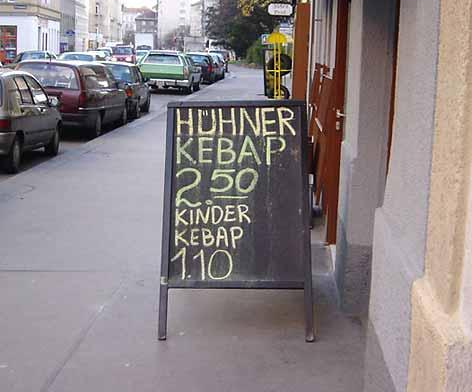
\includegraphics[scale=.55]{material/05Morph-Kebap}
\end{figure}

\end{frame}


%%%%%%%%%%%%%%%%%%%%%%%%%%%%%%%%%%
%%%%%%%%%%%%%%%%%%%%%%%%%%%%%%%%%%
\subsubsubsection{Rektionskomposita}
%\frame{
%\frametitle{~}
%	\tableofcontents[currentsection]
%}


%%%%%%%%%%%%%%%%%%%%%%%%%%%%%%%%%%
\begin{frame}
\frametitle{Rektionskomposita}

\begin{itemize}
	\item Wichtige \textbf{Untergruppe} der Determinativkomposita:
	
	\eal \label{ex:Bsp1} 
        \ex die Linguisten tagen
        \ex die Tagung der Linguisten
        \ex Linguistentagung
	\zl
	
	\eal \label{ex:Bsp2} 
        \ex die Linguisten besteigen den Watzmann
        \ex die Besteigung des Watzmann
        \ex Watzmannbesteigung
	\zl
		 
\end{itemize}


\end{frame}


%%%%%%%%%%%%%%%%%%%%%%%%%%%%%%%%%%
\begin{frame}
\frametitle{Rektionskomposita}

\begin{itemize}
	\item \textbf{deverbale} Nomina (durch Derivation)
	
	\begin{itemize}
		\item[]
		\item tagen \ras Tagung
		\item[]
		\item Verb bestimmt mit wie vielen und mit welchen Argumenten es im Satz erscheint\\
                  (s. Rektion, Subkategorisierungsrahmen)
		
		\begin{itemize}
			\item[]
			\item Tagen in \ref{ex:Bsp1} + Subjekt
			\item[]
			\item besteigen in \ref{ex:Bsp2} + Subject + Objekt
			\item[]
			\item Beziehung zwischen Verb und seinen Argumenten auch innerhalb eines Kompositums
		\end{itemize}
	\end{itemize}
\end{itemize}


\end{frame}


%%%%%%%%%%%%%%%%%%%%%%%%%%%%%%%%%%
\begin{frame}
\frametitle{Rektionskomposita}

\begin{itemize}
	\item Rektionskompositum: \\
	die erste Konstituente in einem deverbalen Rektionskompositum realisiert ein Argument des der zweiten Konstituente zugrunde liegenden Verbs
	
	\begin{itemize}
		\item[]
		\item In \ref{ex:Bsp1}: \emph{Linguist(en)} \ras Subjekt von \emph{tagen}
		\item[]
		\item In \ref{ex:Bsp2}: Watzmann \ras Objekt von besteigen
	\end{itemize}
	
	\ea	 Auto$\cdot$fahrer (jemand fährt Auto), \\
		 Wetter$\cdot$beobachter (jemand beobachtet das Wetter), \\
		 Rotkehlchen$\cdot$gesang (das Rotkehlchen singt)
	\z
		 
\end{itemize}


\end{frame}


%%%%%%%%%%%%%%%%%%%%%%%%%%%%%%%%%%
\begin{frame}
\frametitle{Rektionskomposita}

\begin{itemize}
	\item Es gibt auch Rektionskomposita, in denen die zweite Konstituente ein nicht-deverbales Nomen oder ein Adjektiv ist, denn auch Nomina und Adjektive können Argumente nehmen:
	
	\ea Prüfungsangst (Angst vor der Prüfung), \\
		 Todessehnsucht (Sehnsucht nach dem Tod)
	\z
		 
	\ea staatstreu (dem Staat treu), \\
		 fälschungssicher (vor Fälschung sicher), \\
		 bleifrei (von Blei frei)
	\z
		 
\end{itemize}


\end{frame}


%%%%%%%%%%%%%%%%%%%%%%%%%%%%%%%%%%
\begin{frame}
\frametitle{Rektionskomposita}

\begin{itemize}
	\item \textbf{Rektionskompositum:} \\
	Kompositum, bei dem die \textbf{erste Konstituente ein Argument} (Subj., Akk.-Obj., Dat.-Obj., Gen.-Obj., Präp.-Obj., etc.) der zweiten Konstituente ist.
	\item[]
	\item Bei Nicht-Rektionskomposita besteht keine Argumentrelation.
	\item[]
	\item[] \textbf{ÜB.4}
	
\end{itemize}


\end{frame}


%%%%%%%%%%%%%%%%%%%%%%%%%%%%%%%%%%
%%%%%%%%%%%%%%%%%%%%%%%%%%%%%%%%%%
\subsubsubsection{Possessivkomposita}
%\frame{
%\frametitle{~}
%	\tableofcontents[currentsection]
%}


%%%%%%%%%%%%%%%%%%%%%%%%%%%%%%%%%%
\begin{frame}
\frametitle{Possessivkomposita}

\begin{itemize}
	\item Auch bei Possessivkomposita bestimmt die erste Konstituente die zweite näher.
	\item[]
	\item Das Kompositum bezieht sich aber auf \textbf{eine dritte Entität}, sie sind \textbf{exozentrisch}
	
	\ea \emph{Rot$\cdot$kehlchen} = Vogel, der ein rotes Kehlchen hat, nicht ein rotes Kehlchen ist
	\z
	
	\ea \emph{Rot$\cdot$käppchen} = Person, die eine rote Kappe hat (Märchenfigur), kein Käppchen
	\z
	
	\ea \emph{Lang$\cdot$finger} = Person, die lange Finger hat (= die stiehlt), kein Finger
	\z
	
\end{itemize}


\end{frame}


%%%%%%%%%%%%%%%%%%%%%%%%%%%%%%%%%%
%%%%%%%%%%%%%%%%%%%%%%%%%%%%%%%%%%
\subsubsubsection{Kopulativkomposita}
%\frame{
%\frametitle{~}
%	\tableofcontents[currentsection]
%}


%%%%%%%%%%%%%%%%%%%%%%%%%%%%%%%%%%
\begin{frame}
\frametitle{Kopulativkomposita}

\begin{itemize}
	\item Erste Konstituente \textbf{bestimmt} die zweite \textbf{nicht näher}
	\item[]
	\item Beide Konstituenten sind \textbf{gleichrangig}
	\item[]
	\item Auch aus mehr als zwei Konstituenten bestehend
	\item[]
	\item \textbf{Koordinierende} (= verknüpfende) Beziehung zwischen den Kompositionsgliedern
	\item[]
	\item Bedeutung des Kompositums ergibt sich \textbf{additiv}
	
	\eal 
	\ex süß$\cdot$sauer, nass$\cdot$kalt, rot$\cdot$grün, Fürst-Bischof
	\ex rot-rot-grün
	\zl
	
\end{itemize}


\end{frame}


%%%%%%%%%%%%%%%%%%%%%%%%%%%%%%%%%%
\begin{frame}
\frametitle{Kopulativkomposita}

\begin{itemize}
	\item Konstituenten in Kopulativkomposita \ras \textbf{gleiche Kategorie}
	\item[]
	\item Reihenfolge: prinzipiell frei, aber meistens \textbf{konventionalisiert}
	\item[]
	\item Anderes \textbf{Betonungsmuster} als Determinativkomposita
	
	\ea ein 'blau-'grünes 'Hemd - Kopulativ \\
		 ein 'blaugrünes 'Hemd - Determinativ
	\z
		 
	\item Während bei Determinativkomposita der Nichtkopf betont wird, werden bei Kopulativkomposita alle Konstituenten betont.
	\item[]
	\item[] \textbf{ÜB.5}
\end{itemize}


\end{frame}



%% \frame{
%% \frametitle{Kopulativkomposita}

%% Bei Kopulativkomposita gibt es keinen Kopf:
%% \ea
%% Fürstbischof = Fürst und Bischof gleichzeitig
%% \z

%% \pause
%% Unterschied zwischen \emph{grellweiß} und \emph{schwarz-weiß}.



%% }


\subsubsection{Derivation}


\frame{
\frametitle{Derivation}

\begin{itemize}
\item Komposition = Stamm + Stamm, Derivation = Stamm + Affix.
\pause
\item Beispiele für Regeln:

\medskip

\begin{tabular}{@{}ll@{}}
Beispiel & Regel\\
Erledigung, Beteiligung, Rechnung & N $\to$ V \suffix{ung}$_N$\\
lesbar, essbar, erklärbar & Adj $\to$ V \suffix{bar}$_{Adj}$\\
ungemütlich, unfreundlich, unschön & Adj $\to$ \prefix{un} Adj\\
Schönheit, Freiheit, Falschheit & N $\to$ Adj \suffix{heit}$_N$\\
\end{tabular}

\medskip

\pause
\item Kopf steht wieder rechts (Affixe haben Wortart)
\end{itemize}

}


\subsubsubsection{Selektion}

\frame{
\frametitle{Selektion}

Affixe gehen nicht mit beliebigem anderen Material zusammen,\\
sondern wählen sich ihren Partner aus.
\pause
\begin{itemize}
\item Wortart: \suffix{bar} verbindet sich nur mit Verben\\
      (nicht mit Adjektiven oder Nomina, bis auf unproduktive Ausnahmen)
\pause
\item Phonologische Restriktionen: \suffix{keit} verbindet sich nur mit mehrsilbigen Adjektiven, die
  auf eine unbetonte Silbe enden: \emph{Freundlichkeit}, \emph{Lesbarkeit}, \noword{Schönkeit},
  \noword{Freikeit}.
\pause
\item Bedeutung: \suffix{fach} verbindet sich nur mit Zahlen und Mengenangaben \emph{dreifach},
  \emph{mehrfach}, \noword{schönfach}, \noword{hausfach}
\pause
\item Morphologische Struktur: \gee verbindet sich nur mit morphologisch einfachen Verben
\emph{Gerenne}, \emph{Gehupe}, \noword{Geverkaufe}, \noword{Geanfange}
\end{itemize}


}

\subsubsubsection{Komplexe Verben}

\frame{
\frametitle{Komplexe Verben}

\begin{itemize}
\item Unterscheiden zwei Arten komplexer Verben: \\
Präfixverben (\emph{bestechen}, \emph{verlangen}, \emph{zersägen}) und Partikelverben
(\emph{ankaufen}, \emph{austrinken}, \emph{anlachen})
\begin{itemize}
\item Präfixverben verhalten sich wie Simplizia.
\item Partikelverben müssen in bestimmten syntaktischen bzw.\ morphologischen Umgebungen
  getrennt werden.
\eal
\ex dass Peter das Haus verkauft
\ex Peter verkauft das Haus.
\zl
\eal
\ex dass Peter das Glas austrinkt
\ex Peter trinkt das Glas aus.
\zl
\eal
\ex zersägt, zersägen
\ex ausgetrunken, auszutrinken
\zl

\end{itemize}


\end{itemize}

}


\subsubsection{Nichtkonkatenative Prozesse}

\subsubsubsection{Konversion}

\frame{
\frametitle{Nichtkonkatenative Prozesse: Konversion}


\begin{itemize}
\item Es gibt auch nichtkonkatenative Prozesse. Beispiel \blaubf{Konversion}
\item Wortart des Stammes wird geändert, ohne dass Material hinzugefügt würde.
\eal
\ex schlaf$_V$ $\to$ Schlaf$_N$
\ex grün$_{Adj}$ $\to$ grün$_{V}$
\ex braun$_{Adj}$ $\to$ bräun$_{V}$
\zl
\end{itemize}




}


\subsubsubsection{Kurzwortbildung}


\frame{
\frametitle{Kurzwortbildung und Kontamination}


\begin{itemize}
\item Kurzwortbildung
\eal
\ex Autobus $\to$ Bus
\ex Universität $\to$ Uni
\zl
\pause
\item Kontamination
\eal
\ex jein (jein = ja + nein)
\ex Teuro (teuer + Euro)
\zl


\end{itemize}





}
